 \documentclass[12pt]{article}
%%% ----------------------------------------------------------------------
%\pagestyle{headings}
%%% ----------------------------------------------------------------------
%%% PAQUETES -------------------------------------------------------------
%=-=-=-=-=-=-=-=-=-=-=-=-=-=-=-=-=-=-=-=-=-=-=-=-=-=-=-=-=-=-=-=-=-=-=-=-=
\usepackage[english,activeacute]{babel}
\usepackage{natbib}
\usepackage{comment}
\usepackage{float}
\usepackage[hidelinks]{hyperref}
\usepackage{mathrsfs}
\usepackage{enumitem}
\usepackage[font={small,it}]{caption}
\usepackage{amsmath,amsfonts,amsthm,amssymb}
\usepackage{bm,rotating,multirow,dsfont,graphicx}
\usepackage[usenames,dvipsnames]{color}
\usepackage{url}
\usepackage{multicol}
\usepackage{multirow}
\usepackage[T1]{fontenc}
\usepackage{flafter}
\usepackage{appendix}
\usepackage{subfigure}
\usepackage{xcolor}
\usepackage{soul}
\usepackage{threeparttable}
%%% ----------------------------------------------------------------------
%%% TABLES ---------------------------------------------------------------
%%% ----------------------------------------------------------------------
\makeatletter
\def\hlinewd#1{%
	\noalign{\ifnum0=`}\fi\hrule \@height #1 %
	\futurelet\reserved@a\@xhline}
\makeatother
%%% ----------------------------------------------------------------------
%%% FORMATO DE PÁGINA ----------------------------------------------------
%=-=-=-=-=-=-=-=-=-=-=-=-=-=-=-=-=-=-=-=-=-=-=-=-=-=-=-=-=-=-=-=-=-=-=-=-=
\addtolength{\oddsidemargin}{-.5in}%
\addtolength{\evensidemargin}{-.5in}%
\addtolength{\textwidth}{.9in}%
\addtolength{\textheight}{.8in}%
\addtolength{\topmargin}{-.7in}%
\setlength{\parindent}{0pt}
\setlength{\parskip}{6pt}
%
\DeclareMathOperator*{\argmax}{arg\,max}
\DeclareMathOperator*{\argmin}{arg\,min}
%
\newcommand\simiid{\mathrel{\overset{\makebox[0pt]{\mbox{\normalfont\tiny\sffamily iid}}}{\sim}}}
\newcommand\simind{\mathrel{\overset{\makebox[0pt]{\mbox{\normalfont\tiny\sffamily ind}}}{\sim}}}
\newcommand{\pr}[1]{\textsf{Pr}\left(#1\right)}
\newcommand{\ind}[1]{\mathbf{1}\left\{ #1 \right\}}
\newcommand\floor[1]{\lfloor#1\rfloor}
\newcommand{\expec}[1]{\textsf{E}\left(#1\right)}
\newcommand{\expe}[1]{\textsf{E}\left(#1\right)}
\newcommand{\var}[1]{\textsf{Var}\left(#1\right)}
\newcommand{\sd}[1]{\textsf{SD}\left(#1\right)}
\newcommand{\cov}[1]{\textsf{Cov}\left(#1\right)}
%
\newcommand{\minus}{\scalebox{0.75}[1.0]{$-\,$}}
\newcommand{\sgn}{\mathrm{sgn}}
\newcommand{\ds}{\displaystyle}
\newcommand{\pt}{\partial}
\newcommand{\dd}{\mathrm{d}}
\newcommand{\lp}{\left(}
\newcommand{\rp}{\right)}
\newcommand{\lb}{\left[}
\newcommand{\rb}{\right]}
\newcommand{\lc}{\left\{}
\newcommand{\rc}{\right\}}
\newcommand{\be}{\begin{eqnarray*}}
\newcommand{\ee}{\end{eqnarray*}}
\newcommand{\bet}{\begin{eqnarray}}
\newcommand{\eet}{\end{eqnarray}}
%
\def\spacingset#1{\renewcommand{\baselinestretch}{#1}\small\normalsize}\spacingset{1}
%
\def\@roman#1{\romannumeral #1}
%
\graphicspath{{./plots/}}

\setlength{\parindent}{0pt}

\begin{document}

\begin{titlepage}
\centering
{
\includegraphics[width=0.125\textwidth]{escudoUN.png}\par}
{\bfseries\LARGE Universidad Nacional de Colombia \par}
\vspace{1cm}
{\scshape\Large Facultad de Ciencias \\ Departamento de Estadística\par}
\vspace{3cm}
{\scshape\Huge CASO 1 - ESTADÍSTICA BAYESIANA\par}
\vspace{0.5cm}
\begin{spacing}
{\Large MODELADO BAYESIANO DE LOS RESULTADOS EN MATEMÁTICAS DE LA PRUEBA SABER 11: UN ESTUDIO DE TENDENCIAS \par}
\end{spacing}
\vfill
\textbf{\Large{Autores:}}
    \vspace{2cm}
    \begin{tabular*}{\textwidth}{@{\extracolsep{\fill}} c c c c}
        &                               &                               & \\
        &                               &                               & \\
        & \Large{Luis Felipe Basto Ruiz} & \Large{Cesar Augusto Prieto S.} & \\
        &                               &                               & \\
        & \large{lbastor@unal.edu.co} & \large{ceprieto@unal.edu.co} & \\
    \end{tabular*}
\vfill
{\Large \today \par}
\end{titlepage} 


\vspace{2mm}
  
\par

\tableofcontents %No borrar 
\listoffigures %No borrar
\listoftables %No borrar

\newpage %No borrar

\section{INTRODUCCIÓN}

En este trabajo se analiza el desempeño del componente de matemáticas de la Prueba Saber 11, una evaluación estandarizada de alcance nacional administrada por el Instituto Colombiano para la Evaluación de la Educación (ICFES). Dentro de las diferentes áreas de la prueba, la sección de matemáticas, por las diferentes competencias que llega a medir por sí misma, presenta una buena oportunidad para mostrar, de una manera corta pero efectiva, un panorama general sobre el nivel de preparación de los estudiantes próximos a culminar la educación media en Colombia.\\\\
Partiendo de una base de datos, que abarca la información de los 32 departamentos de Colombia, junto con Bogotá, a través de los periodos correspondientes entre el segundo semestre de 2015 y el segundo semestre de 2023, el objetivo principal de este análisis es modelar y comparar los diferentes resultados en matemáticas por medio del estudio de patrones, gráficos y tendencias que le permitan al lector identificar brechas en el aprendizaje, evaluar políticas educativas y proponer estrategias basadas en evidencia estadística. Para este fin, se aplica un enfoque basado en modelos Bayesianos jerárquicos, que como se podrá apreciar más adelante, a través de simulaciones de Monte Carlo, facilitarán la estimación de parámetros clave, y a su vez, el análisis de la evolución de estos a través del tiempo en función de sus características.



\section{EXPLICACIÓN DEL MODELO}

El modelo utilizado para este análisis es un modelo Bayesiano jerárquico basado en una combinación de distribuciones \textbf{Normal} y \textbf{Gamma Inversa}, adecuado para casos donde tanto la media como la varianza de los datos son inciertas y tratadas como variables aleatorias. Este modelo aprovecha distribuciones previas conjugadas, lo que facilita la derivación de las correspondientes distribuciones posteriores.  

El modelo se define a través de las siguientes relaciones jerárquicas:  

\begin{itemize}
    \item \textbf{Distribución muestral}  
   Se supone que los puntajes de matemáticas $(y_i)$ siguen una distribución Normal con media $(\theta)$ y varianza $\sigma^2$:  
   
   $$
   y_i \mid \theta, \sigma^2 \sim N(\theta, \sigma^2), \quad i = 1, \dots, n.
   $$

    \item  \textbf{Distribución previa de $\theta$ (media condicional en $\sigma^2$)}  
   El parámetro $\theta$ tiene una distribución Normal con media $\mu_0$ y varianza $\sigma^2 / \kappa_0$:  
   
   $$
   \theta \mid \sigma^2 \sim N\left(\mu_0, \frac{\sigma^2}{\kappa_0}\right),
   $$
   
   donde $\kappa_0$ representa la precisión equivalente a un tamaño efectivo de observaciones previas en torno a la media previa $\mu_0$.

    \item \textbf{Distribución previa de  $\sigma^2$ (varianza)}  
   El parámetro $\sigma^2$ sigue una distribución Gamma Inversa con parámetros de forma $\nu_0 / 2$ y escala $(\nu_0 \sigma_0^2) / 2$:  
   
   $$
   \sigma^2 \sim \text{GI}\left(\frac{\nu_0}{2}, \frac{\nu_0 \sigma_0^2}{2}\right),
   $$
   
   donde $\nu_0$ refleja el tamaño efectivo de una muestra previa y $\sigma_0^2$ es la varianza previa.
\end{itemize}

\subsection{HIPERPARÁMETROS}

Los valores iniciales utilizados en el modelo son:  

\begin{itemize}
    \item $\mu_0 = 50$: Media previa basada en el puntaje promedio esperado de la prueba.  
    \item $\kappa_0 = 1$: Representa una precisión baja equivalente a una observación previa.  
    \item $\nu_0 = 1$: Número de grados de libertad, asociado a una muestra previa mínima.  
    \item $\sigma_0^2 = 10^2$: Varianza previa basada en la desviación estándar típica de la población evaluada.  
\end{itemize}

\subsection{SIMULACIÓN Y AJUSTE DEL MODELO}

El ajuste del modelo se realiza de manera independiente para cada departamento y período, utilizando simulación de Monte Carlo con $B = 10,000$ iteraciones. Esto permite obtener distribuciones posteriores para los parámetros $\theta$ (media) y $\sigma^2$ (varianza), asegurando resultados consistentes y reproducibles.  

Este modelo permite capturar incertidumbre de manera explícita, proporcionando estimaciones robustas y visualmente interpretables, esenciales para comprender las dinámicas educativas en Colombia.  


\section{DESARROLLO DEL CASO}

\subsection{Estimación de parámetros para Bogotá en 2023-2}

El enunciado del primer punto a desarrollar dice lo siguiente: Para Bogotá en 2023-2 ($t=9$), calcule la media posterior, el coeficiente de variación posterior y el intervalo de credibilidad al 95$\%$ de confianza para la media $\theta$, la desviación estándar $\sigma$ y el coeficiente de variación $\zeta=100\,\frac{\sigma}{|\theta|}\%$. Reporte los resultados tabularmente.

Con esto, los pasos a ejecutar son los siguientes:

\begin{itemize}
    \item Ajustar el modelo Bayesiano (Normal-Gamma Inversa-Normal) con los hiperparámetros proporcionados.
    \item Calcular la media posterior, el coeficiente de variación posterior y los intervalos de credibilidad al $95\%$ para la media, desviación estándar y coeficiente de variación.
    \item Reportar los resultados en una tabla.
\end{itemize}

Para resolver este problema, se utilizó un enfoque bayesiano basado en el modelo Normal-Gamma Inversa-Normal, que es particularmente adecuado para contextos donde tanto la media como la varianza de los datos son inciertos. Este modelo permite incorporar información previa (hiperparámetros) junto con los datos observados para actualizar el conocimiento sobre los parámetros de interés.

El análisis se desarrolló en varias etapas:

\begin{itemize}
    \item Selección y Filtrado de Datos
    \item Cálculo de Estadísticos Muestrales
    \item Actualización a un ajuste Bayesiano
    \item Simulación de Monte Carlo
     \item Tabulación de resultados
\end{itemize}

\begin{table}[H]
\centering
\begin{tabular}{lcccc}
\hline
\textbf{Inferencia Bayesiana} & \textbf{Estimación} & \textbf{CV} & \textbf{L. Inf.} & \textbf{L. Sup.} \\
\hline
Media & 55.073 & 0.008 & 54.249 & 55.922 \\
Desviación & 11.994 & 0.025 & 11.418 & 12.597 \\
Coef. de Var & 0.218 & 0.026 & 0.207 & 0.229 \\
\hline
\end{tabular}
\caption{Inferencia Bayesiana sobre $(\theta)$, $(\sigma)$, $(\zeta)$ }
\label{tab:inferencia-bayesiana}
\end{table}


\begin{figure}[H]
    \centering
    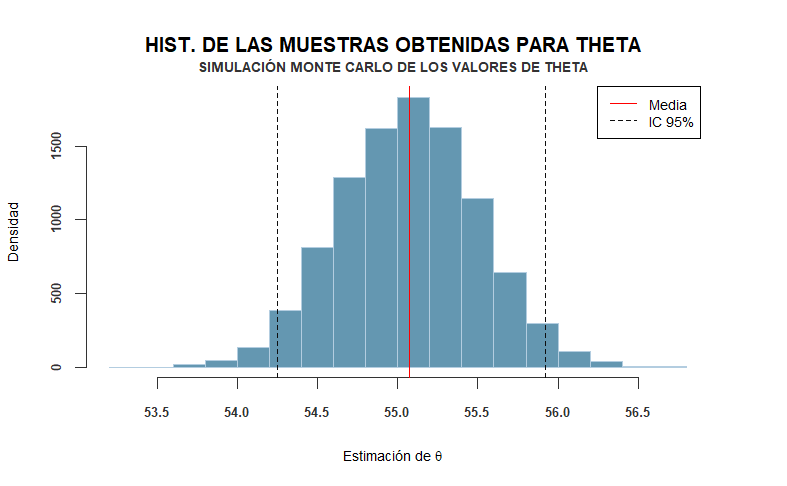
\includegraphics[width=0.8\linewidth]{Imagenes/Histograma-1.png}
    \caption{Histograma para $(\theta)$ Simulación Monte Carlo }
    \label{fig_enter_label}
\end{figure}

Como se puede apreciar, la media posterior $(\theta)$ es de 55.073, y ya que su respectivo coeficiente de variación es muy bajo y a la vez los intervalos de credibilidad no contienen el valor de 50 que se tiene como referencia, se puede decir que con una probabilidad del 95 $\%$, Bogotá en 2023 obtuvo un promedio de puntajes superiores al promedio teórico nacional de 50 puntos. 

\begin{figure}[H]
    \centering
    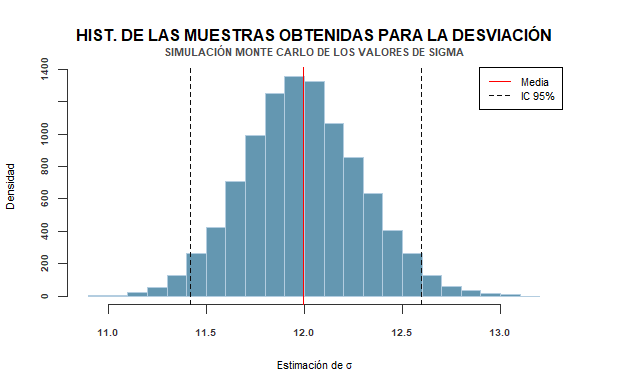
\includegraphics[width=0.8\linewidth]{Imagenes/Histograma-2.png}
    \caption{Histograma para $(\sigma)$ Simulación Monte Carlo }
    \label{fig_enter_label}
\end{figure}

Por otra parte, al concentrarse en la desviación estándar posterior $(\sigma)$, se puede ver que esta es de 11.994, y como su coeficiente de variación asegura buena precisión, por ser muy bajo, y a su vez los intervalos de credibilidad no contienen el valor de 10 establecido para este tipo de pruebas, se concluye entonces que con una probabilidad del 95 $\%$, Bogotá en 2023 obtuvo una desviación superior en sus puntajes con respecto al teórico nacional de 10 puntos. 

\begin{figure}[H]
    \centering
    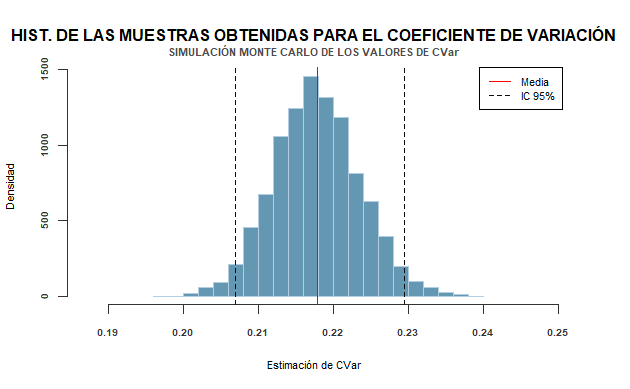
\includegraphics[width=0.8\linewidth]{Imagenes/Histograma-3.png}
    \caption{Histograma para $(\zeta)$ Simulación Monte Carlo }
    \label{fig_enter_label}
\end{figure}

Por último, al revisar el coeficiente de variación $(\zeta)$, se ve que de manera posterior este arroja un valor de 0.218, el cual, al compararse con el estándar esperado de 0.2, se ve que es ligeramente superior, y además de esto, se confirma esta afirmación porque se tienen intervalos de credibilidad que no contienen el valor de 0.2 y un coeficiente de variación de solo 0.026, lo cual da una buena precisión sobre la estimación y permite concluir que con una probabilidad del 95 $\%$, Bogotá en 2023 tuvo una variación en sus puntajes ligeramente superior al 0.2 que se esperaba teóricamente.\\

En general, se puede decir entonces que los resultados muestran que los estudiantes de Bogotá en $t=9$ tuvieron un desempeño promedio superior al estándar nacional, pero con una variabilidad, que aunque sea ligeramente pequeña, si es superior a la esperada. Esto sugiere que Bogotá tiene buen nivel de preparación en matemáticas por encima del esperado, aunque con cierta heterogeneidad dentro de su población estudiantil.\\

De manera adicional, se muestran los histogramas correspondientes a las distribuciones de los valores simulados de $(\theta)$, $(\sigma)$, y $(\zeta)$ para así observar de manera gráfica tanto las estimaciones como su precisión y los intervalos de credibilidad establecidos.\\


\subsection{Ranking de los mejores departamentos en 2023-2}

El enunciado del segundo punto a desarrollar dice lo siguiente: En 2023-2 ($t=9$), elabore el ranking de los cinco departamentos con mejores calificaciones promedio. Para cada uno de estos departamentos calcule la media posterior, el coeficiente de variación posterior y el intervalo de credibilidad al 95$\%$ de confianza para la media $\theta$. Reporte los resultados tabularmente. Además, genere una visualización de estos cinco departamentos mediante un mapa de Colombia que utilice una escala de colores adecuada para representar la media posterior de la media $\theta$.

Con esto, los pasos a ejecutar son los siguientes:

\begin{itemize}
    \item   Calcular la media posterior y otras estimaciones para cada departamento.
    \item  Identificar los cinco departamentos con mejores calificaciones promedio.
    \item  Generar un mapa de Colombia con una escala de colores que represente las medias posteriores.
\end{itemize}

\begin{table}[H]
\centering
\begin{tabular}{lcccc}
\hline
\textbf{Departamento} & \textbf{Estimación} & \textbf{Coef Var} & \textbf{Q2.5\%} & \textbf{Q97.5\%} \\
\hline
Santander & 55.407 & 0.014 & 53.881 & 56.931 \\
Bogotá & 55.073 & 0.008 & 54.249 & 55.922 \\
Huila & 54.659 & 0.022 & 52.354 & 56.970 \\
Boyacá & 54.008 & 0.017 & 52.181 & 55.840 \\
Cundinamarca & 53.850 & 0.010 & 52.778 & 54.945 \\
\hline
\end{tabular}
\caption{Inferencia Bayesiana del Top 5 mejores Departamentos}
\label{tab:top-departamentos}
\end{table}

De acuerdo con la tabla anterior, los cinco mejores departamentos, en términos de las calificaciones promedio, corresponden a los departamentos de Santander, Bogotá, Huila, Boyacá y Cundinamarca.\\

En cuanto a las estimaciones, se ve que los cinco departamentos están por encima del promedio estándar y esto se apoya en el hecho de tener coeficientes de variación muy bajos que hacen que las estimaciones sean más precisas y a su vez, los límites de los intervalos no contienen el valor de 50.\\ 

Ahora, antes de ir sobre el gráfico de los cinco mejores, a modo de curiosidad se anexa el gráfico con todos los departamentos, para ver el escenario global de los puntajes de la prueba. 

\begin{figure}[H]
    \centering
    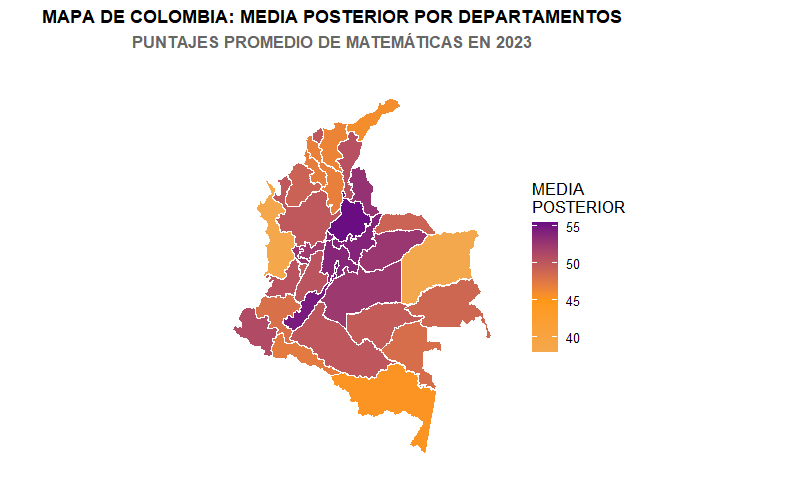
\includegraphics[width=1\linewidth]{Imagenes/MapaColombia1.png}
    \caption{Mapa Colombia todos los departamentos}
    \label{fig_enter_label}
\end{figure}

De aquí, según las convenciones del mapa, se puede ver que entre más oscuro mejores son los puntajes o a su vez si son más bajos se representarían en el mapa como zonas muy claras, lo cual es bastante ilustrativo e informativo para el lector en cuestión, ya que acá va viendo como en toda Colombia los colores van haciendo la escala de color según los resultados.\\

Por otra parte, concentrándose en lo que se quería en particular, se hará el énfasis de los cinco departamentos con mejores puntajes de la prueba.

\newpage

\begin{figure}[H]
    \centering
    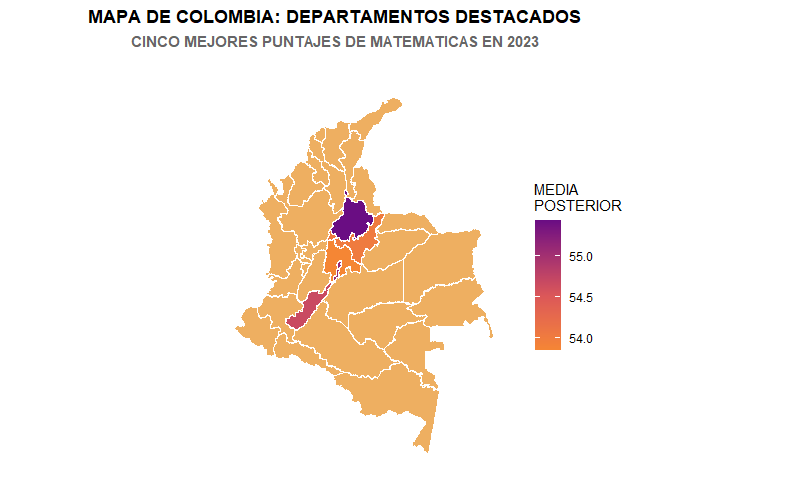
\includegraphics[width=1\linewidth]{Imagenes/MapaColombia2.png}
    \caption{Mapa Colombia Top 5 Mejores departamentos}
    \label{fig_enter_label}
\end{figure}

De aquí, se destaca como el mejor (más oscuro) al departamento de Santander, luego la escala se va degradando de manera respectiva entre Bogotá, Huila, Boyacá y Cundinamarca, dejando así al descubierto de manera visual a los cinco mejores departamentos.


\subsection{Ranking de los peores departamentos en 2023-2}

Para esta parte, se realizará un análisis similar al hecho anteriormente, con la diferencia de que acá se buscará identificar los cinco departamentos con peores calificaciones.

Con esto, los pasos a ejecutar son los siguientes:

\begin{itemize}
    \item  Repetir el proceso anterior para identificar los cinco departamentos con peores calificaciones.
    \item Generar el mapa de Colombia correspondiente con esta característica de interés.
\end{itemize}

A continuación, se presenta la tabla de resultados para los cinco peores departamentos, 

\begin{table}[H]
\centering
\begin{tabular}{lcccc}
\hline
\textbf{Departamento} & \textbf{Estimación} & \textbf{Coef Var} & \textbf{Q2.5\%} & \textbf{Q97.5\%} \\
\hline
La Guajira & 45.832 & 0.025 & 43.583 & 48.067 \\
San Andrés & 45.348 & 0.106 & 35.627 & 54.875 \\
Amazonas & 45.305 & 0.113 & 35.218 & 55.596 \\
Chocó & 38.365 & 0.037 & 35.619 & 41.172 \\
Vichada & 37.916 & 0.162 & 25.757 & 49.948 \\
\hline
\end{tabular}
\caption{Inferencia Bayesiana del Top 5 peores Departamentos}
\label{tab:peores-departamentos}
\end{table}

De acuerdo con la tabla anterior, los cinco peores departamentos, en términos de las calificaciones promedio, corresponden, del puntaje menos bajo al más bajo, a los departamentos de La Guajira, San Andrés, Amazonas, Chocó y Vichada.\\

En cuanto a las estimaciones, se destaca que para el caso de Vichada el coeficiente de variación indica un valor de aproximadamente 16.2 $\%$, lo cual hace que tenga una alta variabilidad que se traduce en una precisión más baja de la estimación. Al tratar de buscar la explicación de esto, se tiene que para este departamento solo se tienen 4 individuos en la muestra lo cual claramente es lo que resulta afectando el valor puntual de la estimación, también se observa esto aunque en una medida más baja para los departamentos de Amazonas y San Andrés.\\

Debido a lo anterior, se puede inferir que La Guajira, Chocó y Vichada reflejarían estar por debajo del promedio estándar establecido de 50 puntos para la prueba, aunque Vichada está muy al límite, con 49.948, y como se mencionó, tiene pocos datos que respalden la calidad de la estimación, podría sugerirse para la investigación tomar más datos para ver mejor la situación, por otra parte, en cuanto a San Andrés y Amazonas, se puede decir que no hay evidencia estadística en contra del supuesto de tener un puntaje igual al promedio estándar de 50 puntos, ya que como se ve el valor de 50 esta contenido dentro de los intervalos de credibilidad.\\

A continuación, se muestra el mapa de Colombia con los cinco departamentos con peores puntajes de la prueba, en este caso, de morado a naranja oscuro, se tendrán respectivamente los puntajes bajos a muy  bajos.

\begin{figure}[H]
    \centering
    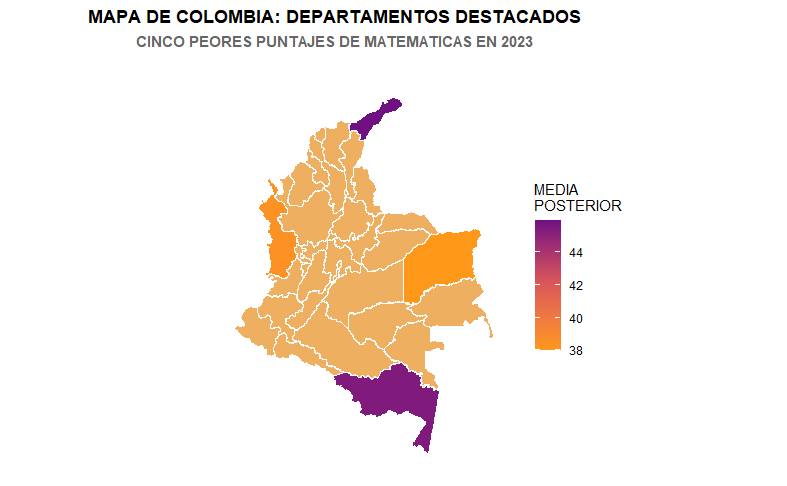
\includegraphics[width=1\linewidth]{Imagenes/MapaColombia3.png}
    \caption{Mapa Colombia Top 5 Peores departamentos}
    \label{fig_enter_label}
\end{figure}


\subsection{Evolución temporal para la media de puntajes en Bogotá}

El enunciado del cuarto punto a desarrollar dice lo siguiente: Para Bogotá en todos los periodos ($t=1,\ldots,9$), calcule la media posterior y el intervalo de credibilidad al 95$\%$ de confianza para la media $\theta$. Presente los resultados mediante una visualización que muestre simultáneamente las medias posteriores y los intervalos de credibilidad.\\

Con esto, los pasos a ejecutar son los siguientes:

\begin{itemize}
    \item Calcular las medias posteriores y los intervalos de credibilidad para Bogotá en cada período ($t = 1$ a $9$).
    \item Generar visualizaciones que muestren la evolución de estos valores a través del tiempo.
\end{itemize}

Luego de ajustar los modelos con respecto a esos diferentes periodos, la tabla para la visualización de estos resultados estaría dada de la siguiente manera:

\begin{table}[H]
\centering
\begin{tabular}{lcccc}
\hline
\textbf{Año} & \textbf{Estimación} & \textbf{Coef Var} & \textbf{Q2.5\%} & \textbf{Q97.5\%} \\
\hline
2015 & 54.149 & 0.007 & 53.374 & 54.941 \\
2016 & 55.621 & 0.007 & 54.917 & 56.341 \\
2017 & 54.098 & 0.007 & 53.377 & 54.835 \\
2018 & 55.408 & 0.009 & 54.455 & 56.386 \\
2019 & 54.813 & 0.009 & 53.824 & 55.797 \\
2020 & 55.607 & 0.010 & 54.480 & 56.724 \\
2021 & 54.342 & 0.007 & 53.570 & 55.137 \\
2022 & 54.640 & 0.008 & 53.813 & 55.464 \\
2023 & 55.073 & 0.008 & 54.249 & 55.922 \\
\hline
\end{tabular}
\caption{Inferencia Bayesiana sobre $(\theta)$ todos los periodos Bogotá}
\label{tab:bogota-periodos}
\end{table}

Como se puede apreciar, las estimaciones para todos los periodos están por encima del estándar de 50 puntos, además de esto, se puede decir que son precisas dado que al hacer el contraste correspondiente con los coeficientes de variación se observa que estos son muy bajos y a la vez ninguno de los periodos tiene un intervalo de credibilidad que contenga el valor poblacional de 50 puntos, así, se puede concluir con una probabilidad del 95 $\%$ que Bogotá en todos los periodos estudiados ha estado por encima del promedio establecido para la prueba.

De manera complementaria, se presenta a continuación un gráfico que refleja las estimaciones por periodo.

\begin{figure}[H]
    \centering
    \includegraphics[width=1\linewidth]{Imagenes/BogotaPorAños1.png}
    \caption{Estimaciones e intervalos de credibilidad sobre $(\theta)$ para Bogotá}
    \label{fig_enter_label}
\end{figure}

Al observar el gráfico, se puede ver de manera muy interesante como los datos muestran por ejemplo dos periodos se destacan con respecto a los demás, estos son los correspondientes a 2016 y 2020. En el primero de estos, se observa un buen puntaje estimado y una banda de credibilidad ligeramente concentrada, lo cual indica buenos puntajes con relativamente baja volatilidad, por otra parte el de 2020 aunque resulto ser bueno y muy cercano al de 2016, tiene un ancho en su intervalo significativamente más amplio, de aquí, una posible explicación podría ser la pandemia, ya que esto represento dificultades logísticas para la presentación del examen que limitaron a muchos estudiantes para poder presentarlo y a su vez la razón de los buenos puntajes se puede decir que tal vez se debieron a que las pruebas se tuvieron que hacer de forma virtual, a su vez, es bastante curioso que para el año 2021 el puntaje haya pasado a ser uno de los tres más bajos en los nueve periodos estudiados, se podría pensar que tal vez por la pandemia hubo una clara incidencia sobre los puntajes, pero que a la vez se midió de mejor manera porque de cierta forma el ICFES estaba más preparado para este examen con respecto al año anterior, estas son tan solo algunas ideas sueltas que se dejan abiertas a los lectores interesados con el fin de que vean como los datos muestran cosas que a simple vista no se pueden ver y con el animo de alimentar la curiosidad que puedan llegar a tener por saber lo que pasa externamente en esos ciertos periodos donde se observan cambios peculiares a la luz de los datos.\\

También de manera adicional, se hace un gráfico extra para ver como se comporta la media de los puntajes de matemáticas en Bogotá a lo largo de los diferentes periodos.

\begin{figure}[H]
    \centering
    \includegraphics[width=1\linewidth]{Imagenes/MapaBogotaPorAño1.png}
    \caption{Mapas sobre la media de los puntajes en Bogotá por año}
    \label{fig_enter_label}
\end{figure}

Aquí de colores oscuros a claros, se observa como de manera respectiva los puntajes van cambiando de mejores a peores con respecto al avance del tiempo.

\subsection{Evolución temporal del Coeficiente de variación en Bogotá}

El enunciado del quinto punto a desarrollar dice lo siguiente:  Para Bogotá en todos los periodos ($t=1,\ldots,9$), calcule la media posterior y el intervalo de credibilidad al 95$\%$ de confianza para el coeficiente de variación $\zeta$. Presente los resultados mediante una visualización que muestre simultáneamente las medias posteriores y los intervalos de credibilidad.

Con esto, los pasos a ejecutar son los siguientes:

\begin{itemize}
    \item Repetir el análisis anterior, pero enfocado en el coeficiente de variación.
    \item Presentar los resultados de manera gráfica.
\end{itemize}

Luego de ajustar los modelos con respecto a esos diferentes periodos, la tabla para la visualización de estos resultados estaría dada de la siguiente manera

\begin{table}[H]
\centering
\begin{tabular}{lcccc}
\hline
\textbf{Año} & \textbf{Estimación} & \textbf{Coef Var} & \textbf{Q2.5\%} & \textbf{Q97.5\%} \\
\hline
2015 & 0.224 & 0.024 & 0.213 & 0.235 \\
2016 & 0.196 & 0.024 & 0.187 & 0.206 \\
2017 & 0.207 & 0.024 & 0.197 & 0.217 \\
2018 & 0.202 & 0.032 & 0.190 & 0.215 \\
2019 & 0.206 & 0.033 & 0.193 & 0.219 \\
2020 & 0.180 & 0.041 & 0.166 & 0.195 \\
2021 & 0.208 & 0.026 & 0.198 & 0.219 \\
2022 & 0.210 & 0.027 & 0.199 & 0.221 \\
2023 & 0.218 & 0.026 & 0.207 & 0.229 \\
\hline
\end{tabular}
\caption{Inferencia Bayesiana de todos los periodos para Bogotá}
\label{tab:bogota-coeficientes-periodos}
\end{table}

De la tabla se puede decir que a modo general durante los periodos estudiados los intervalos de credibilidad tienden a "atrapar" ese valor promedio estándar de 0.2 que se tiene como referencia a nivel poblacional para la prueba, lo cual indica que no hay evidencia estadística que sugiera que dicho valor es diferente a este 0.2 de referencia, sin embargo, para los periodos de 2015 y 2023 se ve que los límites están significativamente por encima de dicho valor, así entonces se concluye que con una probabilidad del 95 $\%$ el coeficiente de variación para la prueba en estos periodos es mayor que el valor de 0.2 esperado, esto indica que habría una mayor volatilidad en los resultados, lo cual se traduce en poder ver tanto puntajes muy bajos como muy altos para ciertos individuos.  \\

Nuevamente, de manera extra se adjunta un nuevo gráfico de las estimaciones junto con sus correspondientes intervalos pero en este caso para el coeficiente de variación. 

\begin{figure}[H]
    \centering
    \includegraphics[width=1\linewidth]{Imagenes/BogotaPorAños2.png}
    \caption{Estimaciones e intervalos de credibilidad sobre $(\zeta)$ para Bogotá}
    \label{fig_enter_label}
\end{figure}

Del gráfico, se ve que al tomar como referencia la línea estándar del valor de 0.2, la mayoría de los periodos en efecto tienden a comportarse como se esperaría, no obstante, es curioso ver como para los años 2015 y 2023 se obtuvieron coeficientes que sobrepasan lo establecido, tal y como se había mencionado al solo ver la tabla, y aun mejor, para el año 2020 se ve que se tuvieron resultados por debajo de esta referencia, lo cual de cierta manera es "extraño" comparando con los demás periodos, pero a la vez si se le trata de dar un sentido que vaya más allá no resulta tan sospechoso al ser el año en el que se presentó el estallido de la pandemia de COVID 19, con esta información se puede complementar lo ya dicho en el punto anterior sobre la estimación de la media y en realidad se ve que este suceso cobra más fuerza como algo que afectó realmente los puntajes de los exámenes y ¿por qué no?, en general la educación colombiana y su medición tal y como se conocía antes de este suceso, de nuevo, cosas que se dejan en el aire gracias a la información que esconden los datos para que cada uno deje volar su imaginación.

Ahora, observemos en el mapa como se comporta el coeficiente de variación de los puntajes de matemáticas en Bogotá en los diferentes periodos con otro gráfico adicional.

\newpage

\begin{figure}[H]
    \centering
    \includegraphics[width=1\linewidth]{Imagenes/MapaBogotaPorAño2.png}
    \caption{Mapas sobre el CV de los puntajes en Bogotá por año}
    \label{fig_enter_label}
\end{figure}

En esta nueva visualización, respectivamente de colores oscuros a claros, se observa como la variación de los puntajes va cambiando de más volátil a menos volátil conforme transcurren los periodos estudiados.

\subsection{Análisis de diferencias ($\eta_{t,k}$ para Bogotá)}

El enunciado del sexto punto a desarrollar dice lo siguiente:  Considere el parámetro $\eta_{t,k} = \theta_t-\theta_{t-k}$, para algún $k=1,\ldots,t-1$. Para Bogotá, calcule la media posterior y el intervalo de credibilidad al 95$\%$ de confianza para $\eta_{9,k}$, para cada $k=1,\ldots,8$. Presente los resultados mediante una visualización que muestre simultáneamente las medias posteriores y los intervalos de credibilidad.

Con esto, los pasos a ejecutar son los siguientes:

\begin{itemize}
    \item Calcular  $\eta_{t,k} = \theta_t-\theta_{t-k}$ para todos los $k$ posibles en cada período.
    \item Reportar las medias posteriores y los intervalos de credibilidad en un gráfico que facilite su interpretación.
\end{itemize}

Luego de ajustar los modelos correspondientes a estas diferencias de los periodos, se muestran los resultados en la tabla a continuación.\\
\begin{table}[H]
\centering
\begin{tabular}{lccccc}
\hline
\textbf{Años} & \textbf{Estimación} & \textbf{Q2.5\%} & \textbf{Q97.5\%} & \textbf{Q0.5\%} & \textbf{Q99.5\%} \\
\hline
2023 - 2015 & 0.923 & -0.231 & 2.068 & -0.602 & 2.380 \\
2023 - 2016 & -0.549 & -1.654 & 0.546 & -2.017 & 0.850 \\
2023 - 2017 & 0.974 & -0.143 & 2.079 & -0.504 & 2.386 \\
2023 - 2018 & -0.335 & -1.650 & 0.964 & -2.063 & 1.349 \\
2023 - 2019 & 0.260 & -1.018 & 1.536 & -1.448 & 1.922 \\
2023 - 2020 & -0.534 & -1.942 & 0.868 & -2.329 & 1.320 \\
2023 - 2021 & 0.731 & 0.679 & 0.785 & 0.661 & 0.801 \\
2023 - 2022 & 0.432 & -0.749 & 1.621 & -1.094 & 1.967 \\
\hline
\end{tabular}
\caption{Inferencia Bayesiana Sobre las diferencias}
\label{tab:diferencias-bayesianas}
\end{table}

De la tabla, al mirar los intervalos de credibilidad, se tiene que para casi todos los periodos no se rechazaría la hipótesis que establece que No existen diferencias significativas entre el último periodo de la prueba con respecto a los demás, ya que estos intervalos contienen al cero, sin embargo, para los periodos 2023-2021 si se aprecia que hay una diferencia significativa entre la media de los puntajes, aquí, dado que el intervalo contiene valores por encima de cero se puede afirmar que con probabilidades del 95 $\%$ y 99$\%$ los puntajes para el año 2023 fueron superiores que para el año 2021.\\

Se muestran también a continuación como complemento histogramas de las diferencias establecidas para observar de manera visual lo anteriormente expuesto. 

\newpage

\begin{figure}[H]
    \centering
    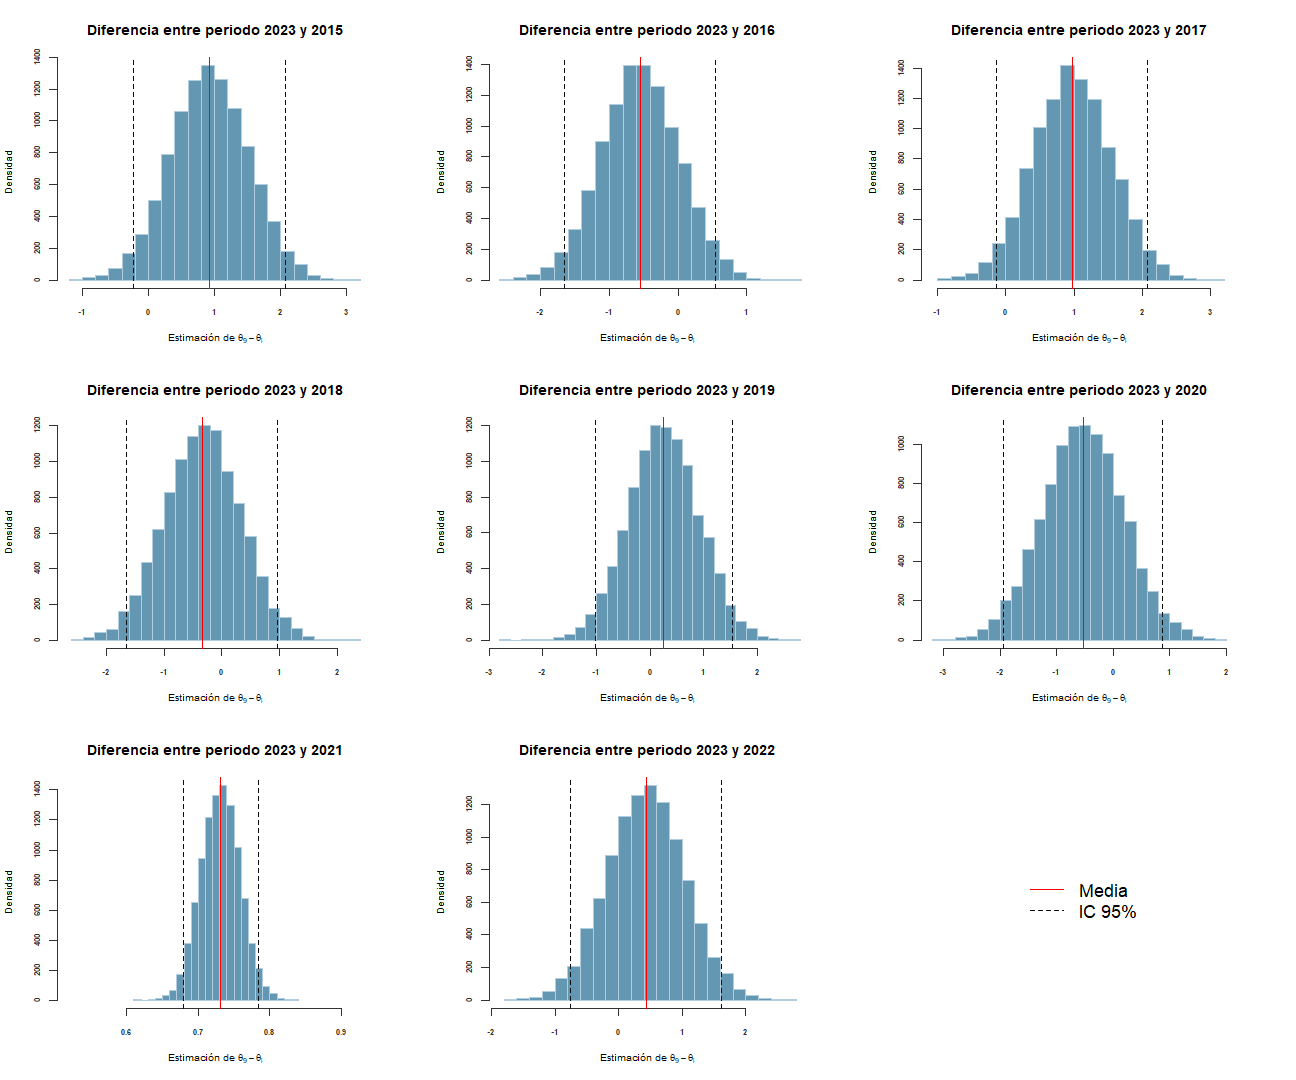
\includegraphics[width=1\linewidth]{Imagenes/GrillaHistogramas.png}
    \caption{Histogramas de las diferencias}
    \label{fig_enter_label}
\end{figure}

Como se aprecia en los histogramas, todos se distribuyen pasando por el cero excepto el intervalo entre $(\theta_9 - \theta_7)$ correspondiente al periodo de comparación 2023-2021, además de que se menciona que gráficamente parece verse más concentrado en sus valores alrededor de la línea roja de estimación.\\

Por último, se muestra un gráfico de las estimaciones y sus correspondientes intervalos de credibilidad.\\ 

\begin{figure}[H]
    \centering
    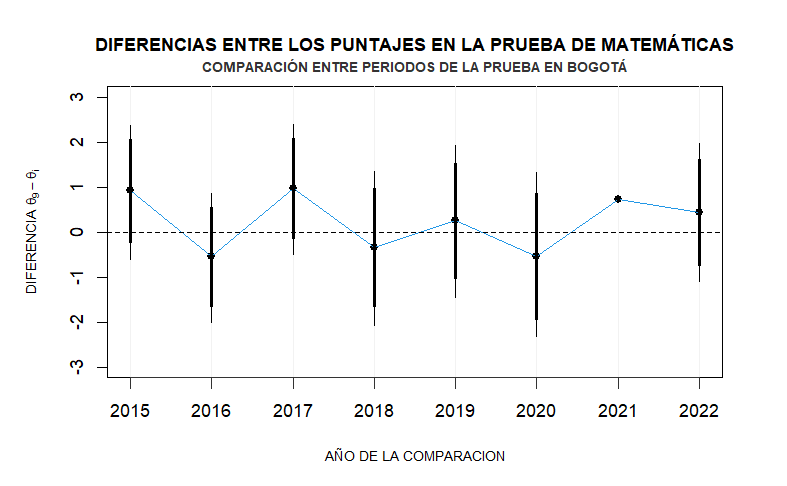
\includegraphics[width=1\linewidth]{Imagenes/Diferenacias.png}
    \caption{Estimaciones e intervalos de credibilidad sobre $(\eta)$ para Bogotá}
    \label{fig_enter_label}
\end{figure}

De este gráfico, tanto a un nivel del 5$\%$ como del 1$\%$ se observa que los intervalos pasan por cero haciendo la salvedad de que para el periodo 2023-2021 si está por encima de esa línea de referencia con lo que se declara que si hay diferencias en esta comparación y además los límites alrededor de la estimación la están "encerrando" dentro de un intervalo muy pequeño de valores lo cual indica una buena precisión. 

\subsection{Procedimiento de agrupamiento Bayesiano}

El enunciado del séptimo punto a desarrollar dice lo siguiente: Para todos los períodos ($t=1, \ldots, 9$), aplique el procedimiento descrito previamente para obtener una segmentación de los 33 departamentos. Para cada período, presentar los resultados mediante un mapa de Colombia, utilizando una escala de colores adecuada en la que los departamentos que pertenezcan al mismo grupo se representen con el mismo color. La visualización debe consistir de 9 paneles dispuestos en un arreglo de $3 \times 3$, todos en una misma página, para facilitar la comparación entre períodos.

Con esto, los pasos a ejecutar son los siguientes:

\begin{itemize}
    \item Implementar el procedimiento descrito usando simulación de Monte Carlo.
    \item Generar las matrices de similitud y aplicar clustering para cada período.
    \item Visualizar los resultados en mapas con un arreglo de $3 \times 3$.
\end{itemize}

El procedimiento descrito a continuación se hace de manera ilustrativa:

\begin{figure}[H]
    \centering
    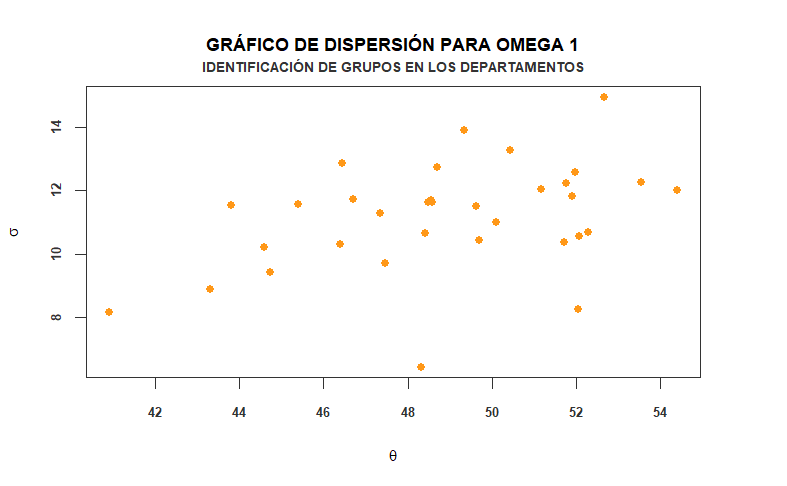
\includegraphics[width=0.7\linewidth]{Imagenes/Dispercion1.png}
    \caption{Dispersión}
    \label{fig_enter_label}
\end{figure}

La figura anterior muestra la dispersión de una de las matrices que se generaron, para así darnos la idea de como se va a plantear el agrupamiento para cada una de las matrices. Luego, y esto solo se realizo una vez, se tomo el agrupamiento jerárquico con el fin de identificar el número de clusters que se pueden formar mediante un dendograma, el cual se muestra en la siguiente figura.

\begin{figure}[H]
    \centering
    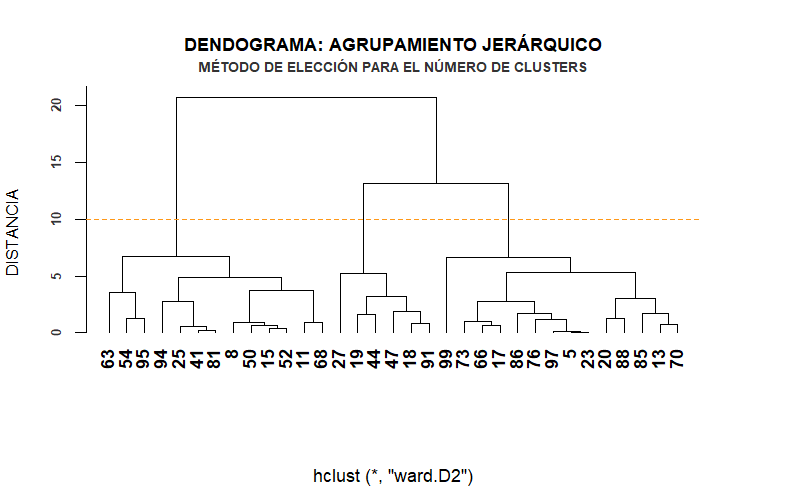
\includegraphics[width=0.7\linewidth]{Imagenes/Dendograma.png}
    \caption{Dendograma}
    \label{fig_enter_label}
\end{figure}

En el Dendograma, se muestra una linea horizontal que parte  a la figura principal en 3 bloques, los cuales representan el número de clusters o grupos por definir, lo ideal sería, hacerlo para cada una de las 10 mil matrices, pero en esta ocasión solo se va a tomar los resultados descritos por este único Dendograma para aplicarlo al resto de matrices y tener resultados más consistentes. Ahora teniendo en cuenta el número de clusters que se pueden formar, en este caos 3, se procede a hacer el agrupamiento con el método de kmeans.

\begin{figure}[H]
    \centering
    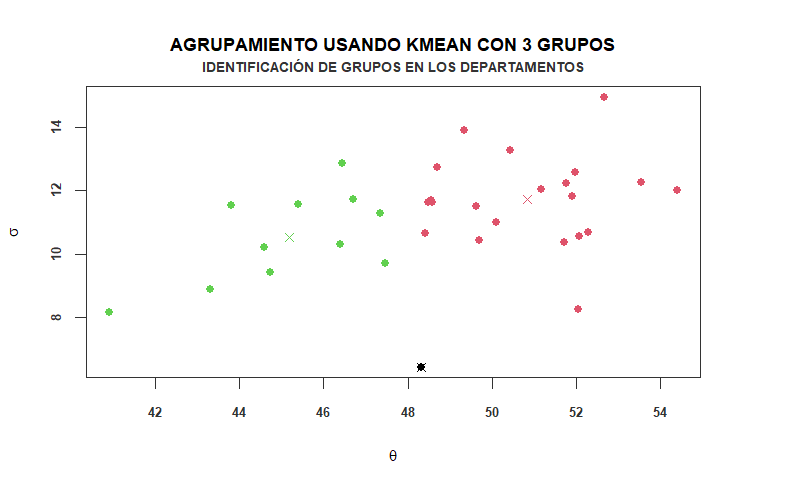
\includegraphics[width=0.7\linewidth]{Imagenes/Dispercion-Kmeans.png}
    \caption{Dispersión-Kmeans}
    \label{fig_enter_label}
\end{figure}

Una vez agrupados con el método de kmeans como se muestra en la figura anterior, se procede a obtener la matriz de similitud al aplicar este procedimiento a cada una de las 10 mil matrices en un tiempo determinado y graficarla mediante un mapa de calor (heatmap).


\begin{figure}[H]
    \centering
    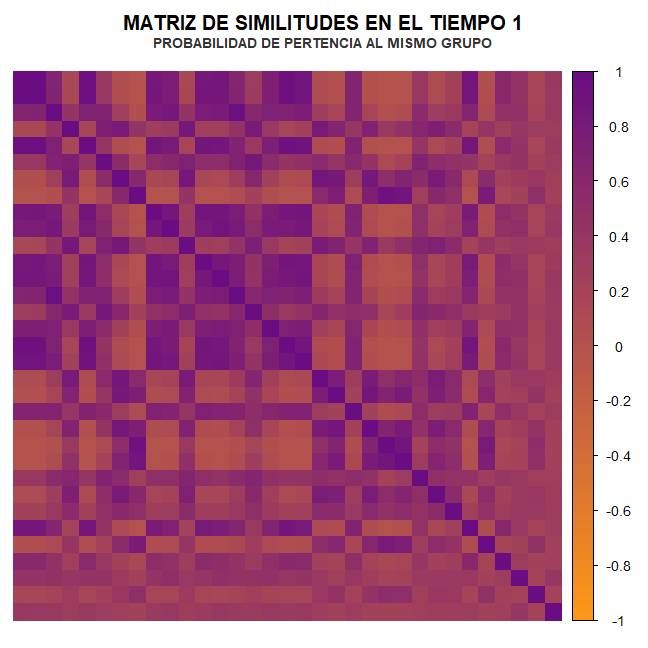
\includegraphics[width=0.7\linewidth]{Imagenes/Mapa-Calor.png}
    \caption{Mapa de Calor}
    \label{fig_enter_label}
\end{figure}

La figura anterior representa la matriz de similitud para el año 2015 aquí representado como el tiempo 1, la cual se calculó a partir de las probabilidades en que dos departamento pertenecían a cierto clúster, de esta forma  se procedió con los datos generados por el código propuesto para resolver el requerimiento, con lo cual, a continuación, generaremos un gráfico donde se muestren las 9 matrices en similitud en el tiempo.
En general para este tipo de diagramas, la interpretación se basará en que de un color oscuro a uno más claro, según el departamento tendrá una mayor o menor probabilidad de pertenecer a cada grupo, de esta manera se puede tener un vistazo gráfico de las coincidencias entre los departamentos.

\newpage

\begin{figure}[H]
    \centering
    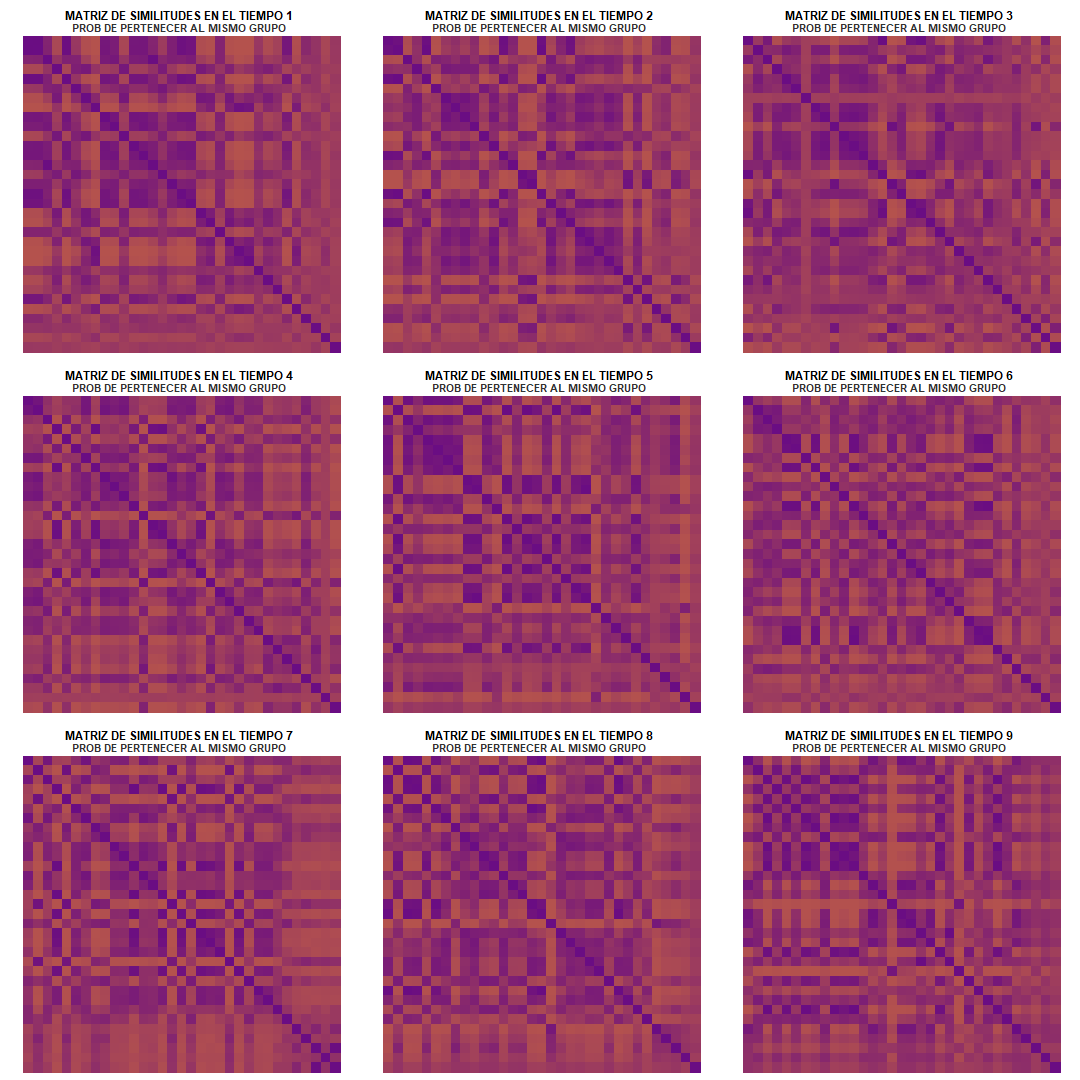
\includegraphics[width=0.9\linewidth]{Imagenes/GrillaHeadMap.png}
    \caption{Grilla Mapa de Calor}
    \label{fig_enter_label}
\end{figure}

Por último, utilizando las matrices de similitudes como entrada de la función Mclust, de la librería mclust se genera la segmentación final (Estimación puntual) teniendo en cuenta las probabilidades contenidas en la matriz de similitud.\\

El procedimiento que se llevo a cabo, planteo realizar el mclust para un primer tiempo o dicho de otra forma sobre la matriz de similitud de un año determinado, para así encontrar el número óptimo de clusters usando el método de ajuste por kernel gaussiano, es decir, usando distribuciones normales multivariadas para esto. A continuación, se muestra la tabla donde se aplica la función a cada matriz y se obtienen los resultados como el BIC y el modelo ajustado a cada matriz de similitud.

\begin{table}[H]
\centering
\begin{tabular}{lccc}
\hline
\textbf{Matriz ID} & \textbf{Num Clústers} & \textbf{Mejor BIC} & \textbf{Modelo} \\
\hline
1 & 5 & 1398.24 & EII \\
2 & 5 & 1498.95 & EII \\
3 & 5 & 1031.56 & EEI \\
4 & 5 & 1647.60 & EEI \\
5 & 5 & 1050.22 & EEI \\
6 & 5 & 1565.98 & EII \\
7 & 5 & 1910.90 & VVI \\
8 & 5 & 1463.61 & EII \\
9 & 5 & 2096.99 & VVI \\
\hline
\end{tabular}
\caption{Métricas de Modelos Mclust por Matriz de Similitudes}
\label{tab:metricas-mclust}
\end{table}

Así, podemos observar que el análisis arroja un máximo de 9 clústers, todos evaluados con diferentes matrices de similitud. Según el BIC, el mejor ajuste se obtiene en la matriz correspondiente al ID 9, con 5 clústers y utilizando el modelo VVI. Este modelo, caracterizado por varianza igual y forma de covarianza variable, sugiere una estructura flexible en los datos, permitiendo capturar variaciones complejas entre los elementos dentro de cada clúster. La elección del modelo VVI indica que las relaciones dentro de los clústers no siguen patrones homogéneos, siendo crucial para representar adecuadamente las características de los datos analizados. Este resultado destaca la importancia de seleccionar tanto la matriz de similitud como el modelo adecuado para optimizar la calidad del agrupamiento.

\begin{figure}[H]
    \centering
    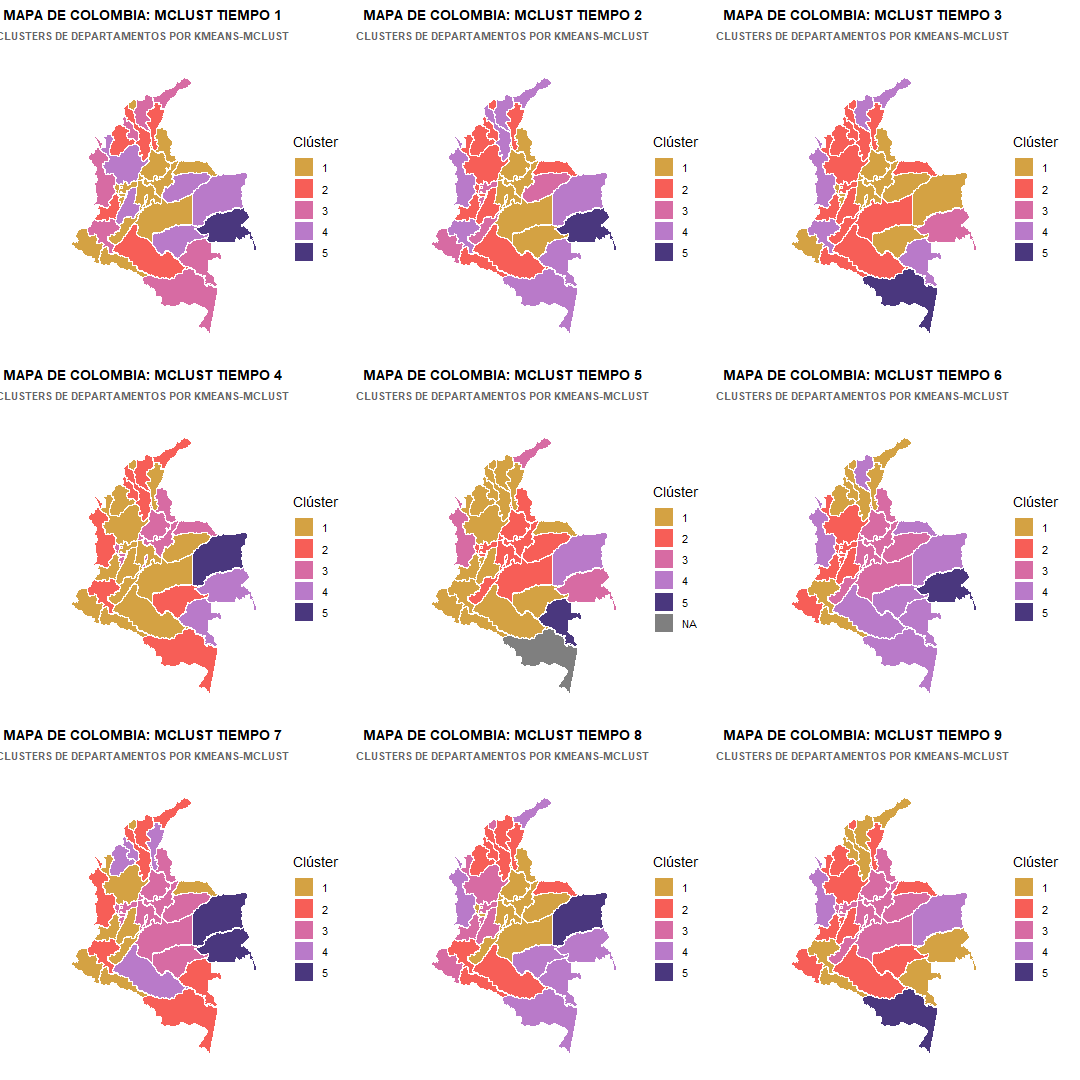
\includegraphics[width=1\linewidth]{Imagenes/GrillaMapaColombia.png}
    \caption{Grilla Mapa Colombia}
    \label{fig_enter_label}
\end{figure}


\subsection{Diagrama de Sankey}

El enunciado del octavo punto a desarrollar dice lo siguiente: Un \textbf{diagrama de Sankey} es una excelente herramienta para visualizar la evolución de un proceso de clustering, ya que puede mostrar cómo los elementos cambian de un grupo a otro a lo largo de diferentes etapas o períodos. Representar la evolución del proceso de clustering obtenido en el numeral anterior mediante un diagrama de Sankey, mostrando cómo los elementos se redistribuyen entre los diferentes grupos a lo largo de los periodos.

\begin{itemize}
    \item Utilizar los resultados de agrupamiento para crear un diagrama de Sankey que muestre la evolución de los grupos a lo largo del tiempo.
\end{itemize}

En un principio nos disponemos a graficar la grilla de diagramas circulares para cada año, con el fin de visualizar la evolución de los grupos a lo largo del tiempo.



\begin{figure}[H]
    \centering
    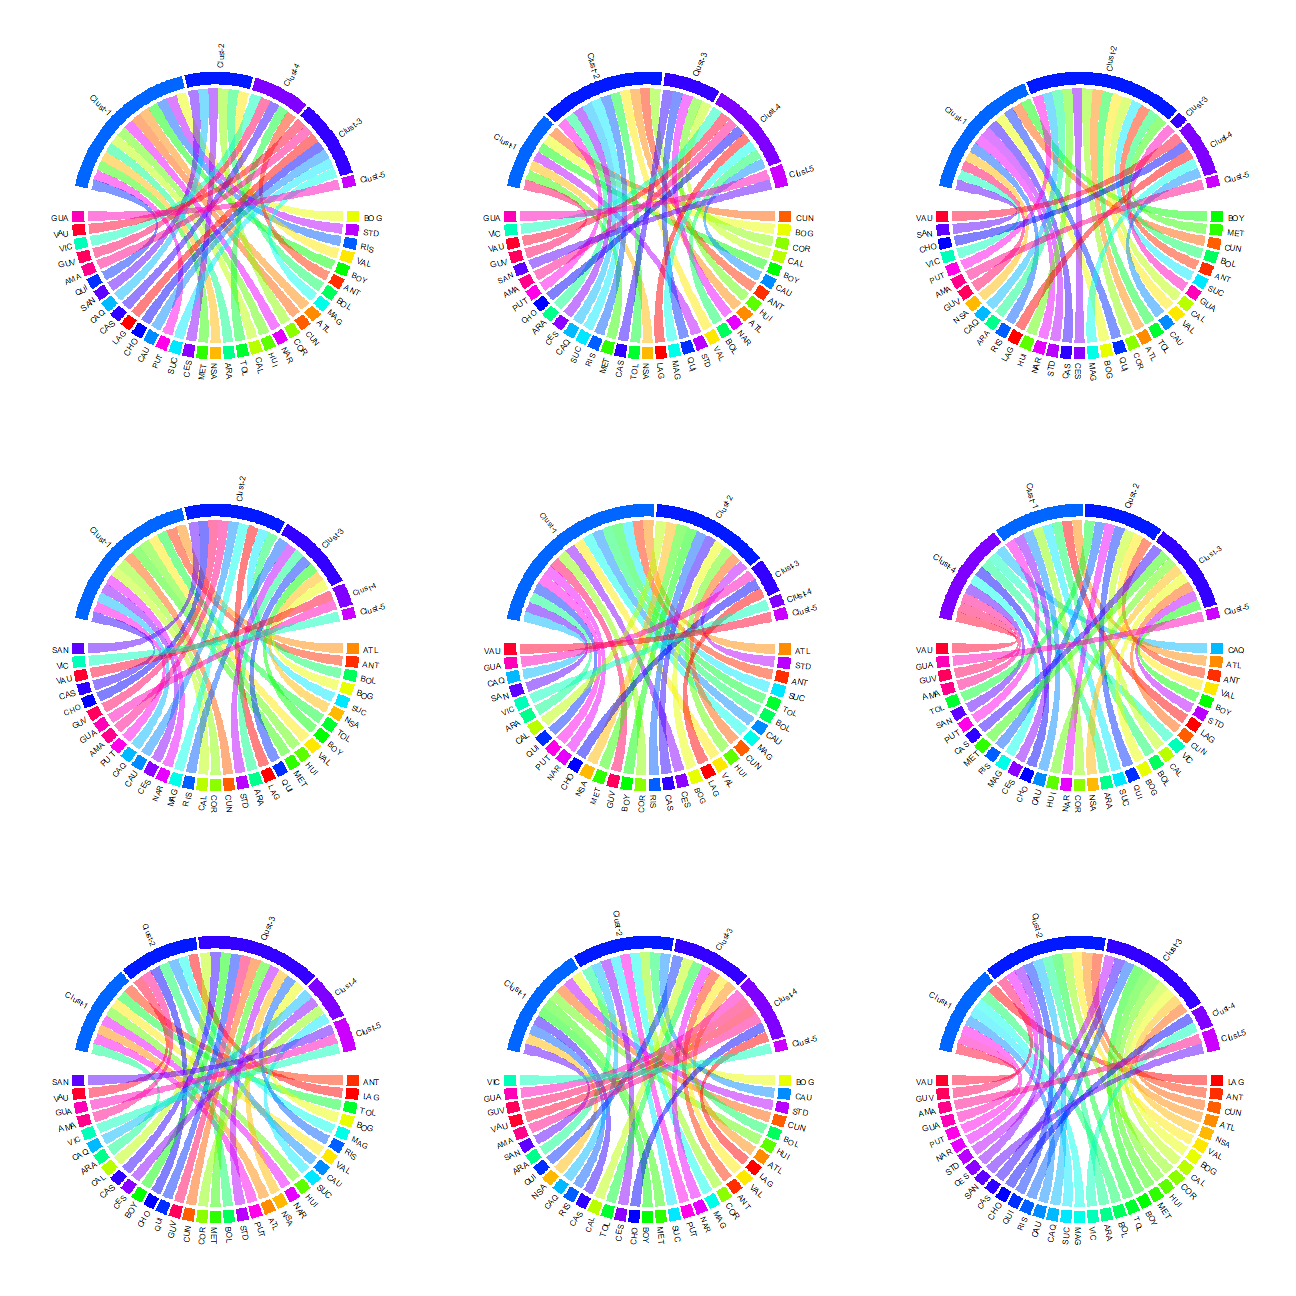
\includegraphics[width=1\linewidth]{Imagenes/GrillaSankey.png}
    \caption{Grilla Diagramas de Sanky}
    \label{fig_enter_label}
\end{figure}

\newpage

La serie de diagramas de Sankey circulares ilustra la evolución de los agrupamientos a lo largo de diferentes escenarios o periodos. Aunque se mantiene la estructura de cinco clústers, los cambios en las conexiones entre departamentos y clústers sugieren variaciones en los patrones de similitud. Esto indica que las características de los datos o las condiciones del modelo impactan significativamente en la configuración de los grupos. Ahora, exploremos el diagrama circular de Sankey para el año 2023, para poder visualizar mejor los datos. 

\begin{figure}[H]
    \centering
    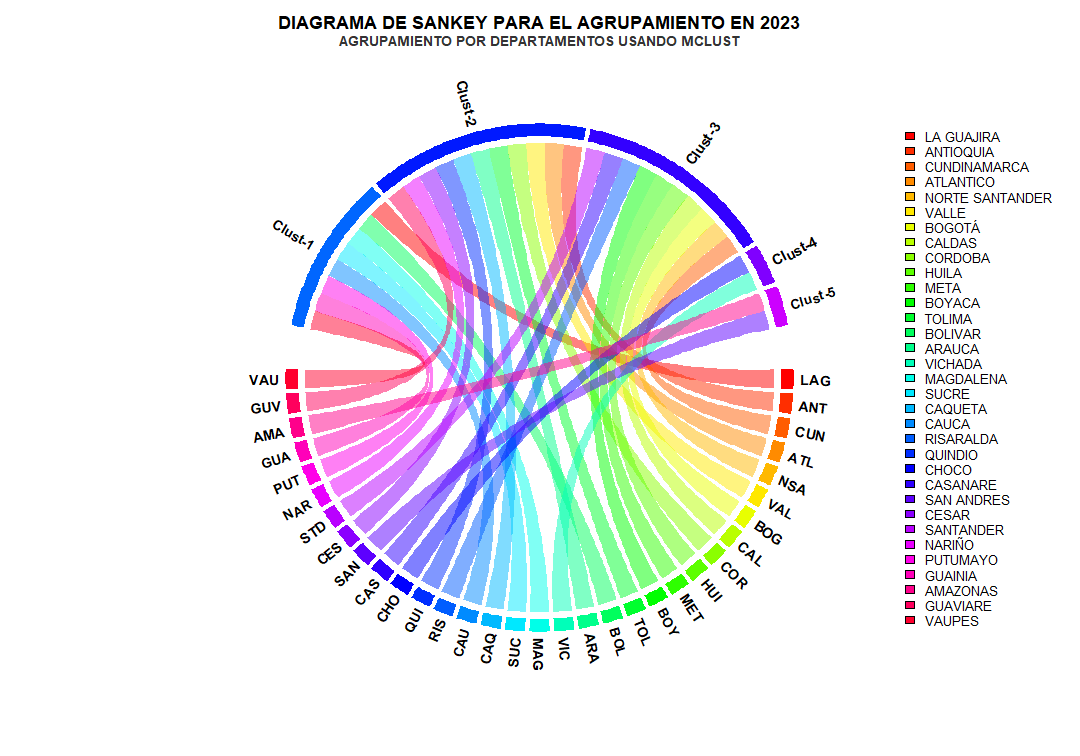
\includegraphics[width=0.8\linewidth]{Imagenes/SankeyIndividual.png}
    \caption{Diagrama Circular de Sankey}
    \label{fig_enter_label}
\end{figure}

El diagrama de Sankey circular muestra la distribución de los departamentos colombianos en cinco clústers principales para el año 2023, según un modelo de agrupamiento basado en Mclust. Se observa que ciertos clústers concentran departamentos con características similares, mientras que otros presentan mayor diversidad en su composición. El uso de conexiones coloridas facilita la identificación de relaciones entre departamentos y clústers, destacando patrones relevantes en el agrupamiento.

\newpage

\subsection{Conclusiones del Análisis}

Como se ha podido ver a lo largo del presente documento, se han hecho ciertos comentarios y análisis en cada uno de los puntos correspondientes para la facilidad del lector en cuestión, ya que mientras se observa el desarrollo estadístico de cada punto, a su vez puede ver las interpretaciones en función de los datos y resultados obtenidos. 

Aclarado esto, para terminar se hace un cierre que deja los resultados que se comentan a continuación.

En primer lugar, viendo los puntajes promedio por departamentos aunque los que están dentro del top superan el promedio, se resalta que tampoco es que lo hagan por mucho, ya que por ejemplo en Santander, que es el que tiene un más alto puntaje para el periodo 2023, este puntaje solo llega a 55.407 lo cual deja bastantes inquietudes por conocer lo que esta detrás de unos resultados que realmente están muy regulares, lo ideal sería acercarse cada vez más a los 100 puntos y no solo en matemáticas sino en las demás áreas del conocimiento, esto a su vez explica el porque de los rendimientos tan pobres que se tienen en pruebas internacionales como por ejemplo las pisa y también el difícil acceso a programas de educación superior dentro de la población colombiana. 

A su vez, se menciona que el análisis en verdad evidenció diferencias significativas en los puntajes de matemáticas entre los diferentes departamentos estudiados, siendo estas más pronunciadas en regiones con un notable acceso limitado a recursos educativos de calidad. Por esta razón, se puede decir que estas brechas están destacando la urgente necesidad de diseñar estrategias focalizadas en los departamentos más afectados que les permitan reducir de cierta manera las desigualdades que tienen en el aprendizaje y a su vez promuevan la equidad educativa comparándose con el resto del país.

También, se puede afirmar que el estudio de patrones fue realmente útil ya que este permitió identificar que por ejemplo, los departamentos que suelen tener mayores tasas de urbanización, al final resultaron presentando un rendimiento consistentemente superior en matemáticas que otros que son rurales. Este hallazgo a modo de comentario adicional, invita a reflexionar sobre el papel de la infraestructura educativa y las oportunidades de formación docente en contextos rurales y urbanos.

Por otra parte, aunque de manera empírica, se podría decir que parece observarse una cierta correlación entre los puntajes en matemáticas y factores como el índice de pobreza, ya que muchos de los departamentos con resultados bajos son de zonas con una economía limitada y hasta reportes de conflictos armados, factores que al final puede afectar en determinada medida la cobertura educativa. Esta relación, para un futuro análisis podría resultar bastante interesante porque podría resaltar la influencia de las condiciones socioeconómicas en el desempeño estudiantil y la importancia de atender estos factores dentro de las políticas públicas.

Para terminar, se puede decir que a partir de los resultados obtenidos, se sugiere, dentro del marco educativo, priorizar estrategias que por ejemplo, incluyan mejores infraestructuras en los colegios, capacitaciones de los docentes para los retos que exige la educación actual y un mayor seguimiento del desempeño estudiantil, esto, con énfasis en departamentos con menor rendimiento, seguramente de esta forma se podrán ver mejoras en el futuro no solo a nivel educativo sino en general en la calidad de vida de todo el país.





\end{document}
